
%% bare_conf.tex
%% V1.4b
%% 2015/08/26
%% by Michael Shell
%% See:
%% http://www.michaelshell.org/
%% for current contact information.
%%
%% This is a skeleton file demonstrating the use of IEEEtran.cls
%% (requires IEEEtran.cls version 1.8b or later) with an IEEE
%% conference paper.
%%
%% Support sites:
%% http://www.michaelshell.org/tex/ieeetran/
%% http://www.ctan.org/pkg/ieeetran
%% and
%% http://www.ieee.org/

%%*************************************************************************
%% Legal Notice:
%% This code is offered as-is without any warranty either expressed or
%% implied; without even the implied warranty of MERCHANTABILITY or
%% FITNESS FOR A PARTICULAR PURPOSE! 
%% User assumes all risk.
%% In no event shall the IEEE or any contributor to this code be liable for
%% any damages or losses, including, but not limited to, incidental,
%% consequential, or any other damages, resulting from the use or misuse
%% of any information contained here.
%%
%% All comments are the opinions of their respective authors and are not
%% necessarily endorsed by the IEEE.
%%
%% This work is distributed under the LaTeX Project Public License (LPPL)
%% ( http://www.latex-project.org/ ) version 1.3, and may be freely used,
%% distributed and modified. A copy of the LPPL, version 1.3, is included
%% in the base LaTeX documentation of all distributions of LaTeX released
%% 2003/12/01 or later.
%% Retain all contribution notices and credits.
%% ** Modified files should be clearly indicated as such, including  **
%% ** renaming them and changing author support contact information. **
%%*************************************************************************


% *** Authors should verify (and, if needed, correct) their LaTeX system  ***
% *** with the testflow diagnostic prior to trusting their LaTeX platform ***
% *** with production work. The IEEE's font choices and paper sizes can   ***
% *** trigger bugs that do not appear when using other class files.       ***                          ***
% The testflow support page is at:
% http://www.michaelshell.org/tex/testflow/



\documentclass[conference]{IEEEtran}

% Some Computer Society conferences also require the compsoc mode option,
% but others use the standard conference format.
%
% If IEEEtran.cls has not been installed into the LaTeX system files,
% manually specify the path to it like:
% \documentclass[conference]{../sty/IEEEtran}
\usepackage[utf8]{inputenc}
\usepackage[T1]{fontenc}
\usepackage[]{algorithm2e}
\usepackage{color}
\usepackage[francais]{babel}
\usepackage[latin1]{inputenc}
	

% Some very useful LaTeX packages include:
% (uncomment the ones you want to load)


% *** MISC UTILITY PACKAGES ***
%
%\usepackage{ifpdf}
% Heiko Oberdiek's ifpdf.sty is very useful if you need conditional
% compilation based on whether the output is pdf or dvi.
% usage:
% \ifpdf
%   % pdf code
% \else
%   % dvi code
% \fi
% The latest version of ifpdf.sty can be obtained from:
% http://www.ctan.org/pkg/ifpdf
% Also, note that IEEEtran.cls V1.7 and later provides a builtin
% \ifCLASSINFOpdf conditional that works the same way.
% When switching from latex to pdflatex and vice-versa, the compiler may
% have to be run twice to clear warning/error messages.






% *** CITATION PACKAGES ***
%
%\usepackage{cite}
% cite.sty was written by Donald Arseneau
% V1.6 and later of IEEEtran pre-defines the format of the cite.sty package
% \cite{} output to follow that of the IEEE. Loading the cite package will
% result in citation numbers being automatically sorted and properly
% "compressed/ranged". e.g., [1], [9], [2], [7], [5], [6] without using
% cite.sty will become [1], [2], [5]--[7], [9] using cite.sty. cite.sty's
% \cite will automatically add leading space, if needed. Use cite.sty's
% noadjust option (cite.sty V3.8 and later) if you want to turn this off
% such as if a citation ever needs to be enclosed in parenthesis.
% cite.sty is already installed on most LaTeX systems. Be sure and use
% version 5.0 (2009-03-20) and later if using hyperref.sty.
% The latest version can be obtained at:
% http://www.ctan.org/pkg/cite
% The documentation is contained in the cite.sty file itself.






% *** GRAPHICS RELATED PACKAGES ***
%
\ifCLASSINFOpdf
  \usepackage[pdftex]{graphicx}
  % declare the path(s) where your graphic files are
  % \graphicspath{{../pdf/}{../jpeg/}}
  % and their extensions so you won't have to specify these with
  % every instance of \includegraphics
  % \DeclareGraphicsExtensions{.pdf,.jpeg,.png}
\else
  % or other class option (dvipsone, dvipdf, if not using dvips). graphicx
  % will default to the driver specified in the system graphics.cfg if no
  % driver is specified.
  % \usepackage[dvips]{graphicx}
  % declare the path(s) where your graphic files are
  % \graphicspath{{../eps/}}
  % and their extensions so you won't have to specify these with
  % every instance of \includegraphics
  % \DeclareGraphicsExtensions{.eps}
\fi
% graphicx was written by David Carlisle and Sebastian Rahtz. It is
% required if you want graphics, photos, etc. graphicx.sty is already
% installed on most LaTeX systems. The latest version and documentation
% can be obtained at: 
% http://www.ctan.org/pkg/graphicx
% Another good source of documentation is "Using Imported Graphics in
% LaTeX2e" by Keith Reckdahl which can be found at:
% http://www.ctan.org/pkg/epslatex
%
% latex, and pdflatex in dvi mode, support graphics in encapsulated
% postscript (.eps) format. pdflatex in pdf mode supports graphics
% in .pdf, .jpeg, .png and .mps (metapost) formats. Users should ensure
% that all non-photo figures use a vector format (.eps, .pdf, .mps) and
% not a bitmapped formats (.jpeg, .png). The IEEE frowns on bitmapped formats
% which can result in "jaggedy"/blurry rendering of lines and letters as
% well as large increases in file sizes.
%
% You can find documentation about the pdfTeX application at:
% http://www.tug.org/applications/pdftex





% *** MATH PACKAGES ***
%
%\usepackage{amsmath}
% A popular package from the American Mathematical Society that provides
% many useful and powerful commands for dealing with mathematics.
%
% Note that the amsmath package sets \interdisplaylinepenalty to 10000
% thus preventing page breaks from occurring within multiline equations. Use:
%\interdisplaylinepenalty=2500
% after loading amsmath to restore such page breaks as IEEEtran.cls normally
% does. amsmath.sty is already installed on most LaTeX systems. The latest
% version and documentation can be obtained at:
% http://www.ctan.org/pkg/amsmath





% *** SPECIALIZED LIST PACKAGES ***
%
%\usepackage{algorithmic}
% algorithmic.sty was written by Peter Williams and Rogerio Brito.
% This package provides an algorithmic environment fo describing algorithms.
% You can use the algorithmic environment in-text or within a figure
% environment to provide for a floating algorithm. Do NOT use the algorithm
% floating environment provided by algorithm.sty (by the same authors) or
% algorithm2e.sty (by Christophe Fiorio) as the IEEE does not use dedicated
% algorithm float types and packages that provide these will not provide
% correct IEEE style captions. The latest version and documentation of
% algorithmic.sty can be obtained at:
% http://www.ctan.org/pkg/algorithms
% Also of interest may be the (relatively newer and more customizable)
% algorithmicx.sty package by Szasz Janos:
% http://www.ctan.org/pkg/algorithmicx




% *** ALIGNMENT PACKAGES ***
%
%\usepackage{array}
% Frank Mittelbach's and David Carlisle's array.sty patches and improves
% the standard LaTeX2e array and tabular environments to provide better
% appearance and additional user controls. As the default LaTeX2e table
% generation code is lacking to the point of almost being broken with
% respect to the quality of the end results, all users are strongly
% advised to use an enhanced (at the very least that provided by array.sty)
% set of table tools. array.sty is already installed on most systems. The
% latest version and documentation can be obtained at:
% http://www.ctan.org/pkg/array


% IEEEtran contains the IEEEeqnarray family of commands that can be used to
% generate multiline equations as well as matrices, tables, etc., of high
% quality.




% *** SUBFIGURE PACKAGES ***
%\ifCLASSOPTIONcompsoc
%  \usepackage[caption=false,font=normalsize,labelfont=sf,textfont=sf]{subfig}
%\else
%  \usepackage[caption=false,font=footnotesize]{subfig}
%\fi
% subfig.sty, written by Steven Douglas Cochran, is the modern replacement
% for subfigure.sty, the latter of which is no longer maintained and is
% incompatible with some LaTeX packages including fixltx2e. However,
% subfig.sty requires and automatically loads Axel Sommerfeldt's caption.sty
% which will override IEEEtran.cls' handling of captions and this will result
% in non-IEEE style figure/table captions. To prevent this problem, be sure
% and invoke subfig.sty's "caption=false" package option (available since
% subfig.sty version 1.3, 2005/06/28) as this is will preserve IEEEtran.cls
% handling of captions.
% Note that the Computer Society format requires a larger sans serif font
% than the serif footnote size font used in traditional IEEE formatting
% and thus the need to invoke different subfig.sty package options depending
% on whether compsoc mode has been enabled.
%
% The latest version and documentation of subfig.sty can be obtained at:
% http://www.ctan.org/pkg/subfig




% *** FLOAT PACKAGES ***
%
%\usepackage{fixltx2e}
% fixltx2e, the successor to the earlier fix2col.sty, was written by
% Frank Mittelbach and David Carlisle. This package corrects a few problems
% in the LaTeX2e kernel, the most notable of which is that in current
% LaTeX2e releases, the ordering of single and double column floats is not
% guaranteed to be preserved. Thus, an unpatched LaTeX2e can allow a
% single column figure to be placed prior to an earlier double column
% figure.
% Be aware that LaTeX2e kernels dated 2015 and later have fixltx2e.sty's
% corrections already built into the system in which case a warning will
% be issued if an attempt is made to load fixltx2e.sty as it is no longer
% needed.
% The latest version and documentation can be found at:
% http://www.ctan.org/pkg/fixltx2e


%\usepackage{stfloats}
% stfloats.sty was written by Sigitas Tolusis. This package gives LaTeX2e
% the ability to do double column floats at the bottom of the page as well
% as the top. (e.g., "\begin{figure*}[!b]" is not normally possible in
% LaTeX2e). It also provides a command:
%\fnbelowfloat
% to enable the placement of footnotes below bottom floats (the standard
% LaTeX2e kernel puts them above bottom floats). This is an invasive package
% which rewrites many portions of the LaTeX2e float routines. It may not work
% with other packages that modify the LaTeX2e float routines. The latest
% version and documentation can be obtained at:
% http://www.ctan.org/pkg/stfloats
% Do not use the stfloats baselinefloat ability as the IEEE does not allow
% \baselineskip to stretch. Authors submitting work to the IEEE should note
% that the IEEE rarely uses double column equations and that authors should try
% to avoid such use. Do not be tempted to use the cuted.sty or midfloat.sty
% packages (also by Sigitas Tolusis) as the IEEE does not format its papers in
% such ways.
% Do not attempt to use stfloats with fixltx2e as they are incompatible.
% Instead, use Morten Hogholm'a dblfloatfix which combines the features
% of both fixltx2e and stfloats:
%
% \usepackage{dblfloatfix}
% The latest version can be found at:
% http://www.ctan.org/pkg/dblfloatfix




% *** PDF, URL AND HYPERLINK PACKAGES ***
%
%\usepackage{url}
% url.sty was written by Donald Arseneau. It provides better support for
% handling and breaking URLs. url.sty is already installed on most LaTeX
% systems. The latest version and documentation can be obtained at:
% http://www.ctan.org/pkg/url
% Basically, \url{my_url_here}.




% *** Do not adjust lengths that control margins, column widths, etc. ***
% *** Do not use packages that alter fonts (such as pslatex).         ***
% There should be no need to do such things with IEEEtran.cls V1.6 and later.
% (Unless specifically asked to do so by the journal or conference you plan
% to submit to, of course. )


% correct bad hyphenation here
\hyphenation{op-tical net-works semi-conduc-tor}
\usepackage{setspace}

\begin{document}

%
% paper title
% Titles are generally capitalized except for words such as a, an, and, as,
% at, but, by, for, in, nor, of, on, or, the, to and up, which are usually
% not capitalized unless they are the first or last word of the title.
% Linebreaks \\ can be used within to get better formatting as desired.
% Do not put math or special symbols in the title.
\title{Développement d'un outil d'édition \\ et de manipulation de réseaux bayésiens}


% author names and affiliations
% use a multiple column layout for up to three different
% affiliations
\author{
\IEEEauthorblockN{R. Agathon}
\IEEEauthorblockA{Telecom Nancy \\
Mail : raphael.agathon@telecomnancy.eu}
\and
\IEEEauthorblockN{V. Wegmann-Serin}
\IEEEauthorblockA{Télécom Nancy \\
Mail: valentin.wegmann-serin@telecomnancy.eu}
\and
\IEEEauthorblockN{C. Simon}
\IEEEauthorblockA{Laboratoire du CRAN \\Mail: christophe.simon@univ-lorraine.fr}
}


% conference papers do not typically use \thanks and this command
% is locked out in conference mode. If really needed, such as for
% the acknowledgment of grants, issue a \IEEEoverridecommandlockouts
% after \documentclass

% for over three affiliations, or if they all won't fit within the width
% of the page, use this alternative format:
% 
%\author{\IEEEauthorblockN{Michael Shell\IEEEauthorrefmark{1},
%Homer Simpson\IEEEauthorrefmark{2},
%James Kirk\IEEEauthorrefmark{3}, 
%Montgomery Scott\IEEEauthorrefmark{3} and
%Eldon Tyrell\IEEEauthorrefmark{4}}
%\IEEEauthorblockA{\IEEEauthorrefmark{1}School of Electrical and Computer Engineering\\
%Georgia Institute of Technology,
%Atlanta, Georgia 30332--0250\\ Email: see http://www.michaelshell.org/contact.html}
%\IEEEauthorblockA{\IEEEauthorrefmark{2}Twentieth Century Fox, Springfield, USA\\
%Email: homer@thesimpsons.com}
%\IEEEauthorblockA{\IEEEauthorrefmark{3}Starfleet Academy, San Francisco, California 96678-2391\\
%Telephone: (800) 555--1212, Fax: (888) 555--1212}
%\IEEEauthorblockA{\IEEEauthorrefmark{4}Tyrell Inc., 123 Replicant Street, Los Angeles, California 90210--4321}}




% use for special paper notices
%\IEEEspecialpapernotice{(Invited Paper)}




% make the title area
\maketitle



\begin{center}
Java, Matlab, inférence, probabilité, graphe probabiliste
\end{center}

% As a general rule, do not put math, special symbols or citations
% in the abstract
\begin{abstract}
The abstract goes here.

\cite{murphyk}
\end{abstract}

% no keywords




% For peer review papers, you can put extra information on the cover
% page as needed:
% \ifCLASSOPTIONpeerreview
% \begin{center} \bfseries EDICS Category: 3-BBND \end{center}
% \fi
%
% For peerreview papers, this IEEEtran command inserts a page break and
% creates the second title. It will be ignored for other modes.
\IEEEpeerreviewmaketitle


\section{Introduction}
% no \IEEEPARstart

Dans le cadre de la recherche, les chercheurs sont régulièrement amenés à utiliser des outils basés sur des graphes probabilistes ou quasi-probabilistes.\\
Par exemple, l'étude de la fiabilité d'un système passe par l'analyse d'un graphe comprenant tous les différents composants du système avec leurs états et probabilités associés - la fiabilité étant l'étude des défaillances des systèmes d'un point de vue statistique -. Les graphes utilisés dans cette étude sont des réseaux bayésiens \cite{kmurphy} \cite{Smail}. Ce sont des modèles probabilistes que l'on trouve sous la forme de graphe acyclique et orientés. Ces modèles utilisent la méthode de l'inférence qui est un procédé permettant de déduire la probabilité d'un événement à partir de celles d'autres événements déjà évalués. Elle repose sur le théorème de Bayes qui repose sur les probabilités conditionnelles et permettant de connaître la probabilité d'un événement:  A sachant B ; lorsque l'on connait la probabilité de A, B, et de B sachant A. \\
Cette usage est souvent accompagné d'une simulation sur logiciel tel que Matlab. Cependant, Matlab ne dispose pas d'outils pratique avec interface graphique permettant de travailler sur les réseaux bayésiens. \\

\tableofcontents
\vspace{0.8cm}
Les chercheurs utilisant principalement l'outil Matlab qui offre un environnement numérique qui donne donc la possibilité de faire des calculs, d'évaluer et de simuler des scénarios. Dans ce cadre, il est nécessaire d'avoir une interface homme machine permettant la création de graphes et de réseaux bayésiens. Cette interface doit aussi nous permettre de manipuler et d'interagir avec les graphes créer et par la suite de faire des calculs d'inférences. Cependant, la création d'interface graphique sous Matlab n'est pas aisée et le logiciel que nous utilisons est donc Java. Ainsi , nous avons une contrainte d'intercommunication entre les deux logiciels. 

\textcolor{red}{
	liste des éléments à rajouter dans la problématique
	\begin{itemize}
	\item contrainte d'intercommunication Java,Matlab
	\item création de réseau bayésien et calcul d'inférence.
	\item présence d'une IHM
	\end{itemize}
}

\\
Afin de répondre au problème donné nous avons choisi de trier tous les logiciels déjà existants puis de surcharger un programme possédant en partie les critères demandés. \\




% An example of a floating figure using the graphicx package.
% Note that \label must occur AFTER (or within) \caption.
% For figures, \caption should occur after the \includegraphics.
% Note that IEEEtran v1.7 and later has special internal code that
% is designed to preserve the operation of \label within \caption
% even when the captionsoff option is in effect. However, because
% of issues like this, it may be the safest practice to put all your
% \label just after \caption rather than within \caption{}.
%
% Reminder: the "draftcls" or "draftclsnofoot", not "draft", class
% option should be used if it is desired that the figures are to be
% displayed while in draft mode.
%
%\begin{figure}[!t]
%\centering
%\includegraphics[width=2.5in]{myfigure}
% where an .eps filename suffix will be assumed under latex, 
% and a .pdf suffix will be assumed for pdflatex; or what has been declared
% via \DeclareGraphicsExtensions.
%\caption{Simulation results for the network.}
%\label{fig_sim}
%\end{figure}

% Note that the IEEE typically puts floats only at the top, even when this
% results in a large percentage of a column being occupied by floats.


% An example of a double column floating figure using two subfigures.
% (The subfig.sty package must be loaded for this to work.)
% The subfigure \label commands are set within each subfloat command,
% and the \label for the overall figure must come after \caption.
% \hfil is used as a separator to get equal spacing.
% Watch out that the combined width of all the subfigures on a 
% line do not exceed the text width or a line break will occur.
%
%\begin{figure*}[!t]
%\centering
%\subfloat[Case I]{\includegraphics[width=2.5in]{box}%
%\label{fig_first_case}}
%\hfil
%\subfloat[Case II]{\includegraphics[width=2.5in]{box}%
%\label{fig_second_case}}
%\caption{Simulation results for the network.}
%\label{fig_sim}
%\end{figure*}
%
% Note that often IEEE papers with subfigures do not employ subfigure
% captions (using the optional argument to \subfloat[]), but instead will
% reference/describe all of them (a), (b), etc., within the main caption.
% Be aware that for subfig.sty to generate the (a), (b), etc., subfigure
% labels, the optional argument to \subfloat must be present. If a
% subcaption is not desired, just leave its contents blank,
% e.g., \subfloat[].


% An example of a floating table. Note that, for IEEE style tables, the
% \caption command should come BEFORE the table and, given that table
% captions serve much like titles, are usually capitalized except for words
% such as a, an, and, as, at, but, by, for, in, nor, of, on, or, the, to
% and up, which are usually not capitalized unless they are the first or
% last word of the caption. Table text will default to \footnotesize as
% the IEEE normally uses this smaller font for tables.
% The \label must come after \caption as always.
%
%\begin{table}[!t]
%% increase table row spacing, adjust to taste
%\renewcommand{\arraystretch}{1.3}
% if using array.sty, it might be a good idea to tweak the value of
% \extrarowheight as needed to properly center the text within the cells
%\caption{An Example of a Table}
%\label{table_example}
%\centering
%% Some packages, such as MDW tools, offer better commands for making tables
%% than the plain LaTeX2e tabular which is used here.
%\begin{tabular}{|c||c|}
%\hline
%One & Two\\
%\hline
%Three & Four\\
%\hline
%\end{tabular}
%\end{table}


% Note that the IEEE does not put floats in the very first column
% - or typically anywhere on the first page for that matter. Also,
% in-text middle ("here") positioning is typically not used, but it
% is allowed and encouraged for Computer Society conferences (but
% not Computer Society journals). Most IEEE journals/conferences use
% top floats exclusively. 
% Note that, LaTeX2e, unlike IEEE journals/conferences, places
% footnotes above bottom floats. This can be corrected via the
% \fnbelowfloat command of the stfloats package.




\section{Analyse des outils existant}
Il existe de nombreuses applications permettant l'édition de réseaux bayésiens. Celles-ci ont toutes leurs spécificités que l'on peut organiser sous forme de catégories. \\
\begin{itemize}
	\item{Langage de programmation :} Il existe des boite à outil pour les réseaux bayésiens dans presque tous les langages de programmation. Les plus connues sont Java Bayes qui est en Java et Bayes Net Toolbox sous Matlab. Il existe d'autres application dont on ne connait pas le langage utilisé. Celle-ci sont la plupart du temps payante ou sont des applications web. La plus connue d'entre elles est BayesiaLab. C'est une application fermée offrant une interface graphique mais sans interaction avec Matlab. BayesiaLab possède un API pour les calculs d'inférence mais cette API ne passe pas par l'interface graphique. \\Les contraintes imposent que l'outil à développer soit sous Java et Matlab en même temps. Dimple est une API qui possède une version Java et une Matlab, mais il n'y a aucune communication entre les deux ce qui ne correspond pas à la problématique et aux contraintes. DynGraph, l'application utilisée est la seul à répondre à cette contrainte. Cette contrainte d'intercommunication est la plus restrictive car l'outil doit permettre l'utilisation de Matlab et de Java en parallèle. Toutes les modifications faites dans l'un des langage doit directement impacter l'autre. \\
	
	\item{Interface graphique :} Parmi toutes les applications connues de réseaux bayésiens, seules 30\% possèdent une interface graphique. La plupart de celles-ci sont en Java comme Java Bayes ou payante comme Bayesialab. Bayes Net Toolbox, CRFtoolbox, DBNbox, OpenGM2 et Probabilistic Modeling Toolkit sont toutes les applications codées sous Matlab. Aucune d'entre elles ne possèdent d'interface graphique.\\ 
	La contrainte de l'interface graphique impose que l'outil en possède déja une ou que celle-ci soit codée par dessus. DynGraph possède une interface graphique en Java Swing, qui offre une grande liberté contrairement à ce qui peut être fait sous Matlab. \\

	\item{Le prix :} l'outil doit être open source et gratuit. La plupart des applications  existantes le sont, mais certaines sont payantes comme BayesiaLab(Bayesialab a été utilisé dans la processus de construction de l'outil de développement de réseaux bayésiens). DynGraph à été codée par des étudiants de notre école, dans le même environnement que le nôtre. Cette application est open source et gratuite et nous pouvons facilement communiquer avec les développeurs. \\
	
	\item{Réseaux bayésiens et Inférence :}Les différentes applications permettent de générer des réseaux bayésiens et de faire de l'inférence sur ceux-ci. Il existe différents algorithme pour le calcul de l'inférence comme JTree et VarElim. DynGraph, l'outil utilisé ne possède aucun outil d'édition de réseaux bayésiens ou de calcul d'inférence. Cet outil permet de construite des graphes pouvant être à nœuds colorés et arcs évalués, orientés ou non. \\
	
\end{itemize}
\\

DynGraph est une application dédié à l'édition et à la manipulation de p-graphes colorés sous Matlab. Cette application Java en open source gratuite assure une interaction dynamique avec Matlab. En revanche elle n'est pas restreinte aux graphes acyclique non colorés et est exempte d'outil d'inférence. 
En restreignant les possibilités de DynGraph dans la construction de graphe, en associant la saisie de probabilités et l'interfacage d'un outil d'inférence alors DynGraph peut être une solution à la problématique. \\
Pour combler ces lacunes,il été choisit de combiner cet outil avec une application Java d'édition de réseaux bayésiens. L'application sélectionnée est Jayes.\\
Jayes est un outil d'édition de réseaux bayésiens, open source et gratuit qui ne dispose pas d'interface graphique.Jayes permet aussi de faire des calculs d'inférences. Parmi les autres applications Java, Jayes possède un code simple de compréhension et permettant une réécriture du code plus facile. \\
Jayes ne dispose d'aucun contrôle sur l'acyclicité des graphes,les dimensions des tables de probabilités ne peuvent être changées qu'une seule fois et il n'y aucun contrôle sur la saisie de données.\\ 


% conference papers do not normally have an appendix


% use section* for acknowledgment
\section{Méthodologie}

Pour arriver à l'objectif, le travail a été divisé en deux parties. Une partie de compréhension et de modification de l'outil DynGraph réaliser par M. Wegmann-Serin et une seconde partie sur la compréhension et l'implémentation des réseaux bayésiens ainsi que des calculs d'inférences. Cette seconde partie a été réalisée par M. Agathon. \\


\subsection{Analyse de l'outil DynGraph}
\vspace{0.3cm} 

DynGraph est un outil permettant la création et l'édition de graphes. Celui-ci est implémenté en java et se lance depuis Matlab.
L'interface (cf fig 1) est composée d'un menu basique et d'une barre composé de boutons permettant d'éditer le graphe. L'éditeur ne permet actuellement que de créer des graphes qui sont orientés ou non, colorés ou non. L'éditeur ne permet pas d'imposer des contraintes lors de la création du graphe telle que l'acyclicité ou la non-évaluation des arcs. Chaque graphe crée est représenté par une liste de nœuds et d'arcs (un arc étant défini par un noeud-début et un noeud-fin ainsi que sa couleur et sa direction).Toute la partie utile aux calculs n'est pas présente : la liste des successeurs et prédécesseurs ou une matrice d'adjacence ou d'incidence. Le côté front-end est implémenté, il s'agit de tous l'aspect visuel. Pour ce qui est du back-end, il s'agit de la communication entre Java et Matlab qui est présente puisque chaque action effectuée sur l'interface - en java - doit être faite en Matlab et inversement. Ainsi, Dyngraph est une IHM permettant l'édition de graphe simple mais pas de réseaux bayésiens et ne permettant pas de faire de calculs d'inférence.Les stratégies possibles pour remédier au problème était de trouver un autre outil offrant plus de fonctionnalités ou d'améliorer Dyngraph.Nous avons choisis de l'améliorer puisque Dyngraph possèdent beaucoup de critères que nous recherchons telle que l'intercommunication Matlab-Java dynamique et le fait que ce soit déjà une IHM. Ainsi, en ajoutant des restrictions offrant la possibilité de créer des graphes acyclique non colorés et en couplant le logiciel avec des outils permettant de faire des calculs d'inférence. Dyngraph se pose alors comme solution convenable pour notre problème.


\begin{figure}[!h]
\begin{center}
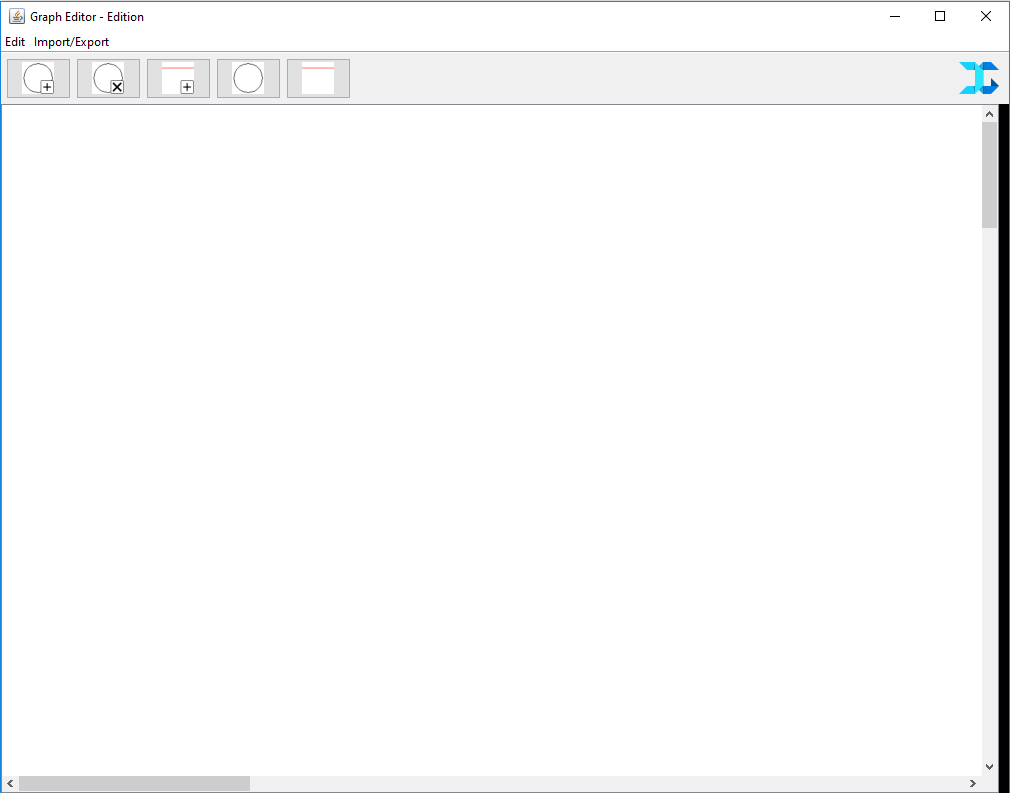
\includegraphics[scale=0.30]{Dyngraph.png}\\
\caption{interface de Dyngraph}
\label{fig 1}
\end{center}
\end{figure}

\subsection{Implémentation des réseaux bayésiens}

Un réseau bayésien est un système représentant la connaissance et permettant de calculer des
probabilités conditionnelles apportant des solutions à différentes sortes de problématiques. \\
La structure de ce type de réseau est simple : un graphe dans lequel les nœuds représentent des
variables aléatoires, et les arcs (le graphe est donc orienté) reliant ces dernières sont rattachées à des
probabilités conditionnelles. \\
Le graphe doit être acyclique : il ne contient pas de boucle. Les arcs représentent des relations
entre variables qui sont soit déterministes, soit probabilistes.
Ainsi, l'observation d'une ou plusieurs causes n'entraîne pas systématiquement l'effet ou les effets qui
en dépendent, mais modifie seulement la probabilité de les observer. \\
\paragraph{Algorithme d'acyclicité \\}
Ainsi, pour transformer un graphe en réseau bayésien il faut vérifier les contraintes d'acyclicité, de directivité du graphe et de non coloration. La coloration peut être enlevée par une simple modification car elle n'impacte pas les données présentes dans le graphe. \\
Contrôler que le graphe est dirigé se fait par une simple vérification sur tous les arcs du graphe.\\
Pour l'acyclicité il existe différents algorithmes de détection de cycle dans un graphe. Des algorithmes comme celui du tri topologique, ou celui de Floyd's Tortoise and Hare sont performants mais nécessites des outils qui implique une totale refonte de la gestion des graphes dans l'outil DynGraph. Cela car ils nécessitent des éléments comme pour chaque nœud une liste des nœuds père et une liste des nœuds fils, ainsi qu'une matrice d'adjacence pour le graphe.C'est élément ne sont pas présent dans l'outil DynGraph.\\
Nous avons donc décidé de coder notre propre algorithme de détection de cycle. Cet algorithme a été spécifiquement construit pour notre cas d'étude : permettre à un utilisateur de savoir si il y a un cycle dans le graphe et si oui afficher la ou les zones à problèmes. \\
L'algorithme repose sur le fait que tous nœud uniquement père ou uniquement fils ne fait pas partie d'un cycle. Par suppression successive de ces nœuds et arcs associes l'algorithme déterminer s'il y a un ou des cycles dans la ou les zones restantes.  \\

 \begin{algorithm}[H]
 \KwData{Graphe G contenant une liste de nœuds et une liste d'arcs}
 \KwResult{liste des nœuds à problème : N}
 N liste de nœuds initialiser avec les noeuds de G\;
 A liste d'arcs initialiser avec les arcs de G\;
 test = True\;
 \While{test = True}{
 	Ra liste d'arcs initialement vide\; 
 	Rp liste des nœuds père, initialement vide\; 
 	Rf liste des nœuds fils initialement vide\; 
 	Rnpf liste des nœuds non père et non fils initialement
 	vide\;
 	test = False\;
 	\ForAll{Arc a dans A }{
 		Ajout du noeud head à la liste Rp\;
 		Ajout du noeud tail à la liste Rf\;
	} 	
 	\EndFor
	\ForAll{Node n dans N }{
		Ajout des nœuds non présent dans l'intersection entre Rp et Rf dans Rnpf\;
	}
	\EndFor 
	\If{Rnpf de taille non nulle}{
		test = True\;
		\ForAll{Arc a dans A}{
			\If{Si un des nœuds de a appartient à Rnpf}{
			Ajout de l'arc a dans la liste Ra\;	 
			}
		}
		Suppression des arcs de Ra dans la liste d'arcs A\;
		Suppression des nœuds de Rnpf dans la liste de nœuds  N\; 
	}	  
 }
\caption{Algorithme de détection de cycle}
\end{algorithm}
\vspace{0.3cm}
Cet algorithme permet de détecter la présence de cycle dans un graphe et permet d'identifier les nœuds inscrits dans un cycle. L'algorithme à une complexité en O(max(n,a)) avec n le nombre de nœud et a le nombre d'arc .Il est possible que certains nœuds, non présent dans un cycle soient inscrits dans les nœuds à problème. Cela car ils sont à l'intérieur d'un ou plusieurs cycle et sont donc classé comme nœuds à problème. La Figure 2 \textcolor{green}{ (si toujours figure 2) } présente 2 cycles. Le nœud présent entre les 2 cycles est considéré comme nœud à problème car  il fait la jonction entre 2 cycles.\\
Cet algorithme utilise iniquement les outils présents dans DynGraph ce qui le rend compatible extrêmement compatible avec cette application\\

\paragraph{Transformation du graphe en réseau bayésien \hfill }
\\ Comme cela est écrit plus haut, le graphe présent dans l'interface DynGraph ne contient aucune information permettant de faire des calculs à partir d'éléments du graphe. Le graphe n'est présent que pour la partie graphique. Il permet à l'interface graphique de générer l'affichage.\\
Deux méthodes ont éte envisagées pour la construction de réseaux bayésiens. \\

\subparagraph{Surcharger le graphe de l'outil DynGraph  \hfill } \\
Cette méthode est la première à laquelle nous avons pensé. Par surcharger il faut comprendre que pour chaque nœud il doit être ajouté : 
\begin{itemize}
\item la liste des nœuds pères 
\item la liste des nœuds fils
\item une table de probabilités 
\end{itemize}
Ainsi que toutes les fonctions et procédures pour que ces différents éléments se mettent à jour automatiquement. \\
De plus comme il est écrit dans la partie III-A l'outil d'édition de réseaux bayésiens est une extension de l'outil DynGraph. C'est pour cela que nous n'avons pas choisi cette méthode car elle implique d'énormes modifications sur le code existant. \\

\subparagraph{Ajouter un graphe de réseau bayésien en parallèle du graphe de l'outil DynGraph \hfill }
\\ Cette seconde méthode est celle qui est implémentée. Les réseaux bayésiens et le calcul d'inférence ont été ajoutés via l'ajout de l'outil Jayes (éditeur de réseaux bayésiens, Java, open source, sans interface graphique). \\
Cette seconde méthode nous permet de ne pas surcharger l'outil initial. Ainsi, si le graphe n'est pas un réseau bayésien, le graphe reste identique. Si le graphe est un réseau bayésien, le graphe visible est celui de DynGraph et en back-end il y a le graphe de Jayes.\\
Lors de la transformation en réseau bayésien. Il y création du graphe de Jayes. 

 \begin{algorithm}[H]
 \KwData{Graphe G contenant une liste de nœuds et une liste d'arcs}
 \KwResult{Graphe de réseau bayésien R}
 N liste de nœuds initialiser avec les noeuds de G\;
 A liste d'arcs initialiser avec les arcs de G\;
 test = True\;
 \ForAll{Node n dans N}{
 	Création du nœud dans graphe R\;
 	Ajout des états True et False pour le nouveau noeud de R\;
 }
 \EndFor
 \ForAll{Arc a dans A}{
 	Ajout du nœud père dans la liste des nœuds père du fils\; 
 }
 \EndFor 
\caption{Algorithme de transformation de graphe}
\end{algorithm}
\vspace{0.3cm}
Après cette étape le graphe réseau bayésien est valide. Toutes les tables de probabilités ont la bonne taille et il ne reste plus qu'à les remplir.

\subsection{Implémentation des probabilités}
Dans un réseau bayésien chaque nœud possède une table de probabilités. Cette table possède un nombre de lignes et de colonnes dépendant d'un certain nombre de paramètres. \\
Le nombre de lignes dépend des différents états que peuvent prendre les variables des nœuds parents de ce nœud. Ce nombre est égal au produit du nombre d'états de chaque nœud parent peut prendre. Si un nœud à 3 nœuds pères, le premier à 2 états, le second et le troisième à 3 états, il y aura 2*3*3 = 18 lignes. Le nombre de colonne, dépend du nombre d'état du nœud. Ainsi chaque case du tableau contient la probabilité que le nœud soit dans un état sachant que les nœuds pères sont dans un certain état.\\
En plus de cette contrainte sur le nombre de lignes et de colonnes, il y a des contraintes sur les valeurs entrées en paramètre. Premièrement il doit y avoir le bon nombre de valeurs et la somme des valeurs sur une ligne doit être égal à 1. Cette dernière contrainte est une contrainte probabiliste. \\  
Une table de probabilité est considérer comme valide lorsque toutes  

\subsection{Calcul de l'inférence}
Le calcul de l'inférence repose sur l'algorithme de l'arbre de jonction \textcolor{green}{mettre une référence https://pdfs.semanticscholar.org/a8d0/f785991019484a64b530849127aca798a9b1.pdf}. Cet algorithme est présent dans l'outil Jayes. Pour pouvoir l'utiliser sans problème il suffit de vérifier que tous les nœuds du graphe ont bien leur table de probabilités valide. 

\subsection{Découpage de l'édition de réseaux bayésiens \hfill}
\\
Éditer un réseau bayésiens impose certaines contraintes sur le graphe comme son acyclicité mais aussi des modifications dynamiques liées à toutes évolutions de celui-ci.Ajouter ou supprimer un arc ou un nœud entraine des modifications sur les dimensions d'au moins une table de probabilités. \\
Pour minimiser ces problèmes de modifications dynamiques et minimiser le nombre de calculs liés aux contraintes, il a été choisi de découper l'édition et l'utilisation de réseaux bayésiens en plusieurs étapes. Ces étapes correspondent aux pratiques utilisateur  : une partie qualitative qui correspond à  l'édition du graphe, une partie quantitative pour la saisie des probabilités et une partie simulation pour les calculs d'inférences. \\

\paragraph{Partie qualitative : édition du graphe \\} \\
Cette étape est celle présente dans l'outil DynGraph. L'utilisateur à la possibilité de créer le graphe qu'il souhaite, acyclique ou non. Durant cette étape aucun réseau bayésien n'est instancié car  l'outil ne sait pas si l'utilisateur veut transformer son graphe en réseau bayésien. Si une transformation est demandée, l'algorithme de détection de cycle est lancé. Cette méthode de découpage fait qu'il n'y a qu'un seul appel à l'algorithme de détection de cycle. Sinon chaque événement sur la structure du graphe induirait une vérification de l'acyclicité. \\

\paragraph{Partie quantitative : saisie probabilités \\ }
Dés lors que le graphe est transformé en réseau bayésien, tout retour à l'étape précédente invalide le réseau bayésiens. Si des nœuds et des arcs sont ajoutés ou supprimés, certaines tables de probabilités changent de dimensions qui rend leurs anciennes valeurs fausse. La table de probabilité de chaque nœud dépend de ses états et des différents états que peuvent prendre ses nœuds parent. Cette construction de table est faite durant la transformation du graphe. La table est automatiquement initialiser avec le bon nombre de colonnes et de lignes. \\
L'ajout de probabilités se fait nœud par nœud. Chaque modification d'une table de probabilités n'est prise en compte que si pour chaque ligne, la somme des valeurs est égale à 1. 
Un passage à l'étape de calcul d'inférence n'est validé que si tous les nœuds ont une table valide. \\

\paragraph{Partie simulation : calculs d'inférences \\}
Les calculs d'inférence ne nécessite pas de contrôle sur les paramètres rentrés. Si un cas d'inférence est invalide, c'est le calcul qui le montrera. Le calcul de l'inférence repose uniquement sur une bonne construction du réseau bayésien. 


\subsection{Modification de l'interface graphique }

Une fois la production du code terminé, les nouvelles fonctionnalités doivent être incorporée dans l'interface. Ce qui a été introduit en premier fut la création de réseaux bayésiens car il s'agit du point de départ de l'analyse scientifique.

\begin{figure}[!h]
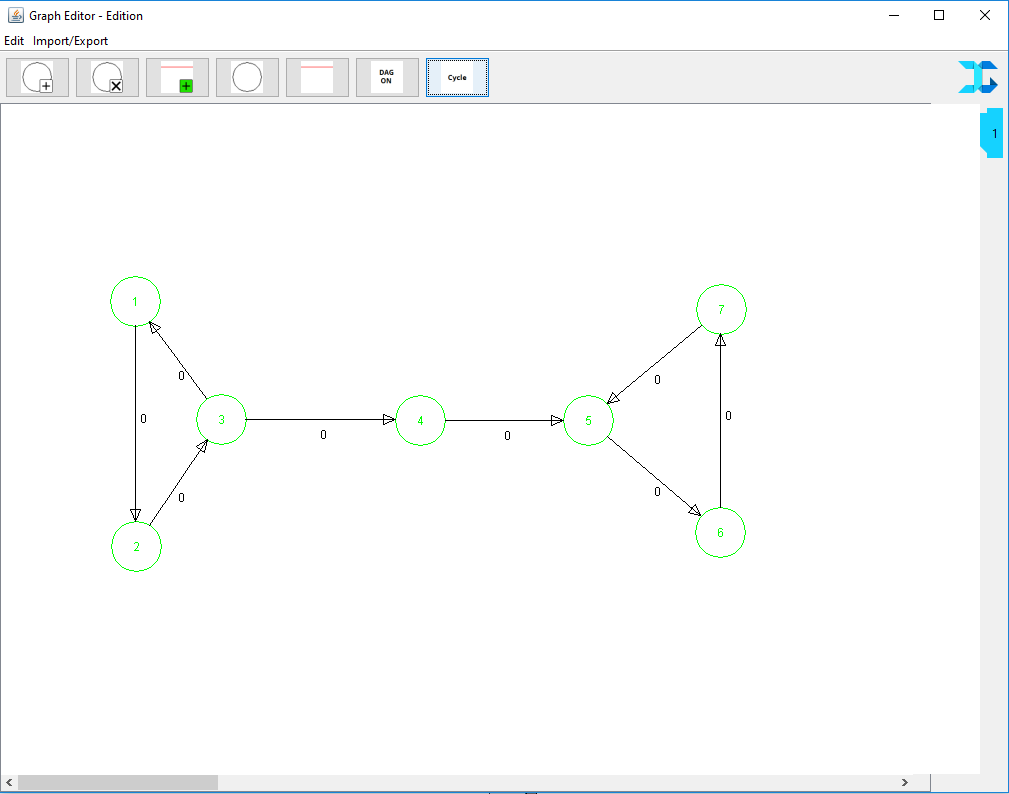
\includegraphics[scale=0.3]{Cycle.png}
\label{fig 2}
\caption{présence de cycle}
\end{figure}

Cette étape est la première dans le processus d'étude. Viens ensuite la phase de mise en place des probabilités. L'utilisateur sélectionne les noeuds un par un et remplie la table des probabilités associée.

\begin{figure}[!h]
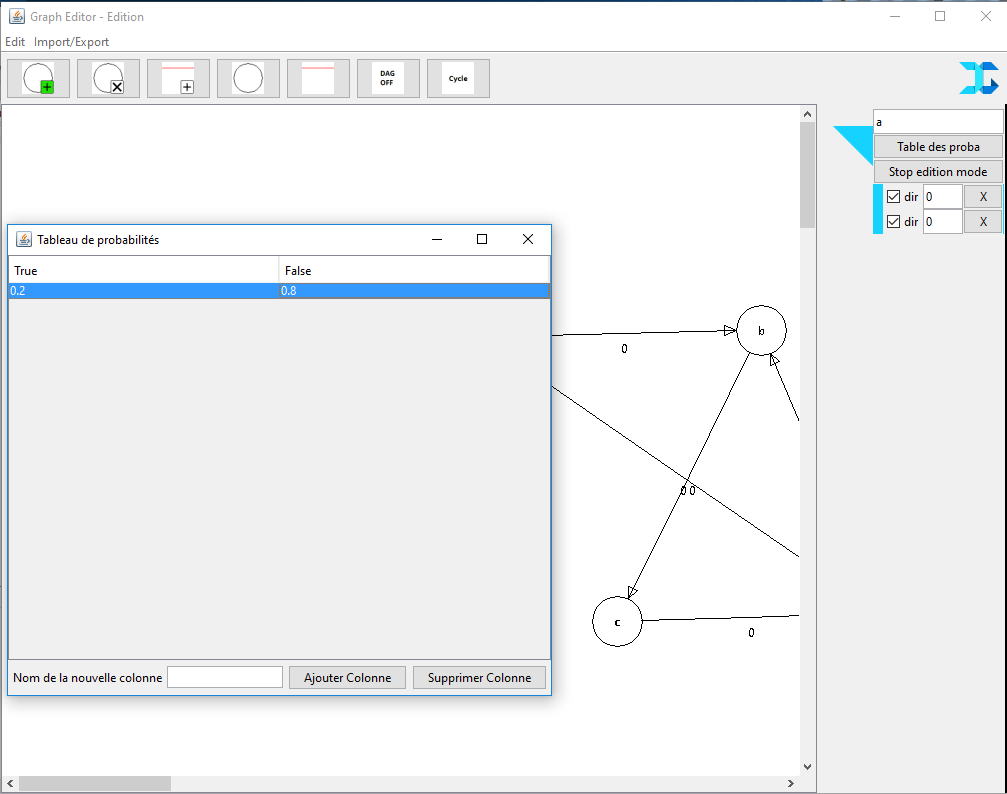
\includegraphics[scale=0.3]{Proba.png}
\label{fig 3}
\caption{table de probabilité}
\end{figure}

Enfin viens la dernière phase qui est celle du calcul des inférences où l'utilisateur aura le choix de lancer une simulation et en choisissant quel événement sont sûrs.\\

Nous avons choisis de découper le processus en trois étape : la création du graphe, la mise en place de probabilité et le calcul d'inférence. Le but de cette découpe est de réduire le nombre de contrôle effectué à chaque modification du graphe. Du fait que l'on utilise des réseaux bayésiens qui possèdent de fortes contraintes - acyclique, dirigé, non-coloré -,le nombre de contrôle à effectuer à chaque fois que l'on modifie le graphe serait lourd. Ainsi, n'effectuer les contrôles qu'une seule fois après avoir fini d'éditer le graphe permet de réduire ce nombre. De plus, les utilisateurs i.e les chercheurs ont l'habitude de créer le graphe et de ne pas le modifier par la suite, d'ajuster les probabilités et enfin de faire les calculs d'inférences nécessaires.

\subsection{Communication entre Matlab Java}
Subsection text here.


\section{Résultats}
	L'outil créer permet l'édition de réseau bayésiens tous en conservant les possibilité qu'offre l'outil DynGraph. Les graphes de réseau bayésien et les calculs d'inférence sont fonctionnels mais peuvent être optimisés. 

\section{Conclusion}

	L'objectif de notre projet à été de créer un outil Matlab et Java pour l'édition de réseaux bayésiens. Cet outil s'ajoute en extension de le l'outil DynGraph.\\
	

\section{Remerciements}
Nous souhaitons adresser nos remerciements aux personnes nous ayant aider dans la rédaction
de cet article, en particulier à M.Simon, notre encadrant de PIDR qui a su nous éclairer dans l'avancée de notre projet. \\
Nous remercions aussi M.Moulet et M.Domingez les créateurs de DynGraph de nous avoir permis d'utiliser leur outil et pour  l'aide qu'il nous ont apporté tout au long de notre projet. 

\section{annexe}

% trigger a \newpage just before the given reference
% number - used to balance the columns on the last page
% adjust value as needed - may need to be readjusted if
% the document is modified later
%\IEEEtriggeratref{8}
% The "triggered" command can be changed if desired:
%\IEEEtriggercmd{\enlargethispage{-5in}}

% references section

% can use a bibliography generated by BibTeX as a .bbl file
% BibTeX documentation can be easily obtained at:
% http://mirror.ctan.org/biblio/bibtex/contrib/doc/
% The IEEEtran BibTeX style support page is at:
% http://www.michaelshell.org/tex/ieeetran/bibtex/
%\bibliographystyle{IEEEtran}
% argument is your BibTeX string definitions and bibliography database(s)
%\bibliography{IEEEabrv,../bib/paper}
%
% <OR> manually copy in the resultant .bbl file
% set second argument of \begin to the number of references
% (used to reserve space for the reference number labels box)
\bibliographystyle{plain}
\bibliography{./pidr}

\cite{Matlab}
\cite{jayes}




% that's all folks

\end{document}


